\documentclass{article}
\usepackage{graphicx}

\begin{document}

\title{Meuse Data Set Interpolation Exercise}
\author{Yin Cheng Ng}

\maketitle

%\begin{abstract}
%\end{abstract}
\section{Introduction}
We explored various interpolation tools to interpolate soil Cadmium concetration as provided in 
the Meuse data set. The models that were investigated are Ordinary Least Square (OLS) regression, 
kernel ridge regression (KRR), Gaussian process (GP), multi-task Gaussian process (MGP) and Bayesian 
neural network (BNN). The models were compared based on 10-fold cross-validated root mean square error 
(RMSE) and mean absolute error (MAE). MGP with soil Zinc concetration as co-variable has the lowest 
cross-validated RMSE and MAE of all models. However, kernel ridge regression has the lowest RMSE and MAE 
among models with no co-variable.

\section{Task description and data set}
The key task is to build a model that can interpolate the topsoil cadmium concentration at unmeasured 
locations, given a set of existing measurements.
\subsection{Data set}
We investigated the Meuse river data set provided in the 'sp' R package. The variables of our key interest 
are the following:
\begin{itemize}
	\item \textbf{x, y} - The 'Easting' and 'Northing' map coordinates of the measurements of 
		interest. The coordinate system used follows the Dutch Rijksdriehoek system.
	\item \textbf{cadmium} - The topsoil cadmiumm concentration, measured in ppm. This variable 
		was incremented by 0.2 compared to the raw measurement, as explained in the description 
		of Meuse data set. This is the target interpolation variable. 
		Refer to Figure \ref{logcad-map} for spatial distributions.
	\item \textbf{copper, lead, zinc} - The topsoil copper, lead and zinc concentrations (in ppm).
		These variables are highly correlated to the topsoil cadmium concentration, and were 
		investigated as covariables in MGP. The Pearson correlation coefficients of the 
		log-concentrations with respect to cadmium log-concentration are tabulated in 
		Table \ref{corr-table}.
\end{itemize}
\subsection{Data pre-processing}
The 'x' and 'y' coordinate variables in the training data set were standardized. 
They each have zero sample mean and variance of approximately one. In addition, the top-soil metal 
concentrations were transformed with base-10 log function for convenience. The original measurements 
have support from zero to infinity.

\begin{figure}[!htbp]
    \centering
    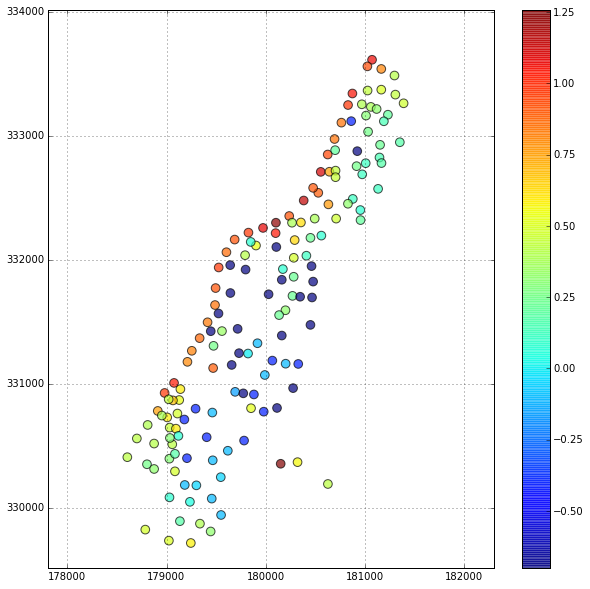
\includegraphics[width=3in]{figures/logcadmium-map.png}
    \caption{Measured log-concentration of topsoil cadmium at various x-y coordinates.}
    \label{logcad-map}
\end{figure}


\begin{figure}[!htbp]
    \centering
    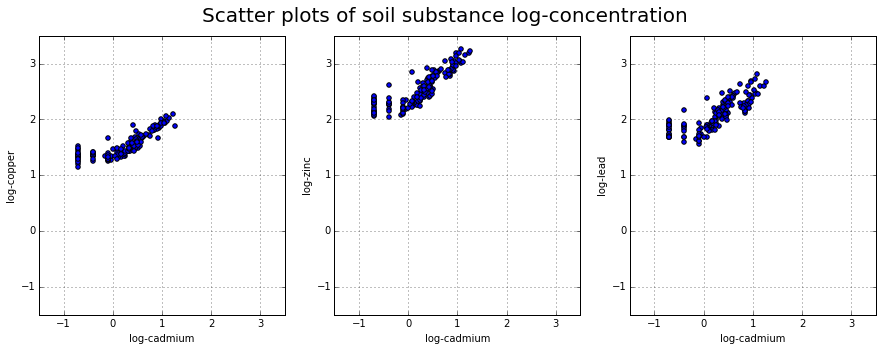
\includegraphics[width=5in]{figures/measurements-scatter.png}
    \caption{Scatter plots of copper, lead and zinc log-concentrations with respect to cadmium log-concentration.}
    \label{measurements-scatter}
\end{figure}

\newpage

\begin{table}[]
\centering
\begin{tabular}{|l|c|c|c|c|}
\hline
        & Cadmium & Copper & Zinc & Lead \\ \hline
Cadmium & 1.0     & 0.84   & 0.86 & 0.81 \\ \hline
Copper  &         & 1.0    & 0.90 & 0.84 \\ \hline
Zinc    &         &        & 1.0  & 0.97 \\ \hline
Lead    &         &        &      & 1.0  \\ \hline
\end{tabular}
\caption{Pairwise Pearson correlation coefficients of topsoil log-concentration measurements.}
\label{corr-table}
\end{table}

\newpage

\section{Models}
We investigated the following models for interpolation of topsoil cadmium concentration. 
Note that target variable in the training data set was centered before model fitting. For predictions, 
the mean of the initial target variable in the training data set was added to the model output, and the 
sum was raised to the power of ten to yield outputs comparable to the original measurements in the Meuse 
data set (i.e., $10^{f_{model} + \mu_{f_{train}}}$ where $f$ is the target variable).
\begin{itemize}
	\item \textbf{OLS Regression (OLS)} - Ordinary least square regression.
	\item \textbf{Kernel Ridge Regression (KRR)} - Kernel ridge regression with Gaussian kernels. 
		Hyperparameters selected through 10-fold cross-validation over a 2-D grid with 
		increment of 0.025 in each dimension.
	\item \textbf{Gaussian Process (GP)} - Gaussian process regression with the Gaussian kernel 
		(also known as the squared-exponential kernel) and Gaussian likelihood. The 
		hyperparameters were selected by maximizing the log-marginal likelihood over the 
		training data set.
	\item \textbf{Cokriging/Multi-task GP (MGP)} - Multi-task GP regression with the Gaussian kernel.
		We investigated using Zinc, Copper and Lead log-concentrations as covariables. The models 
		are referred to as MGP-Zn, MGP-Cu and MGP-Pb respectively. The hyperparameters were 
		selected by maximizing the log-marginal likelihood. In cross-validation, all measurements 
		of the covariable were included in the training data at all time.
	\item \textbf{Bayesian Neural Network (BNN)} - Bayesian neural network trained with the 
		Probabilistic Backpropagation algorithm proposed in 
		\footnote{http://jmlr.org/proceedings/papers/v37/hernandez-lobatoc15.pdf}. Architecture 
		with 2 fully-connected hidden layers of 50 units and 60 units were investigated. 
		The models are referred to as BNN-50 and BNN-60 respectively (BNN-50 has 50 hidden units  
		in each hidden layer, BNN-60 has 60 hidden units in each hidden layer).
\end{itemize}

\subsection{Evaluation metrics}
The models were compared based on 10-fold cross-validated RMSE and MAE. The results are reported in the 
results and discussions section.\\

Note that GP, MGP and BNN provides predictive distributions as outputs while OLS and KRR only provides 
point predictions. For GP, MGP and BNN, the model performance was evaluated based on their predictive means.

\subsection{Software}
Python was the software of choice in the investigation. The OLS and KRR models were fitted with 
implementations in scikit-learn library \footnote{www.scikit-learn.org}, GP and MGP were fitted using 
the excellent GPy library \footnote{https://github.com/SheffieldML/GPy} and 
BNNs were fitted using research code from the author of the original paper \footnote{https://github.com/HIPS/Probabilistic-Backpropagation}.

\section{Results and discussions}
The cross-validation results of the models are presented in Table \ref{result-table}. Among all the 
models, MGP-Zn performed the best. However, among the models with no covariable, KRR performed the best 
while other models, with the exception of OLS, are also competitive.\\

The relatively large difference between RMSE and MAE among models with no covariable suggests that 
there may be outliers. This is verified through inspecting the histograms of residuals in 
Figure \ref{residual}. There is one residual with magnitude greater than 15 among models with no 
covariable.\\

\begin{table}[!htbp]
\centering
\begin{tabular}{|l|r|r|}
\hline
 & RMSE & MAE \\ \hline
OLS & 3.487 & 2.078 \\ \hline
KRR & 2.515 & 1.511 \\ \hline
GP & 2.807 & 1.632 \\ \hline
MGP-Zn & 1.569 & 1.056 \\ \hline
MGP-Cu & 1.902 & 1.177 \\ \hline
MGP-Pb & 2.098 & 1.357 \\ \hline
BNN-50 & 2.714 & 1.520 \\ \hline
BNN-60 & 2.876 & 1.587 \\ \hline
\end{tabular}
\caption{10-fold cross-validated RMSE and MAE.}
\label{result-table}
\end{table}

\begin{figure}[!htbp]
    \centering
    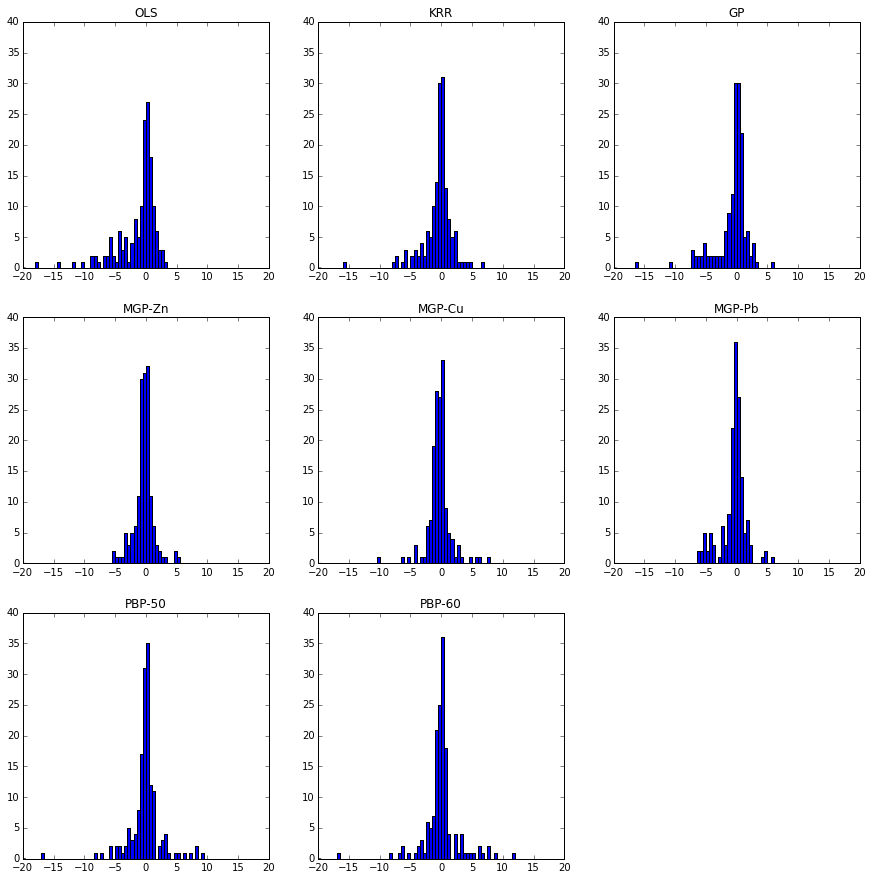
\includegraphics[width=5in]{figures/model-residuals.png}
    \caption{Histogram of cross-validation residuals for all models. The y-axis denotes 
    the frequency count.}
    \label{residual}
\end{figure}


\end{document}
